%% LyX 2.1.4 created this file.  For more info, see http://www.lyx.org/.
%% Do not edit unless you really know what you are doing.
\documentclass[english]{IEEEtran}
\usepackage[LGR,T1]{fontenc}
\usepackage[latin9]{inputenc}
\usepackage{amsmath}
\usepackage{graphicx}

\makeatletter

%%%%%%%%%%%%%%%%%%%%%%%%%%%%%% LyX specific LaTeX commands.
\DeclareRobustCommand{\greektext}{%
  \fontencoding{LGR}\selectfont\def\encodingdefault{LGR}}
\DeclareRobustCommand{\textgreek}[1]{\leavevmode{\greektext #1}}
\DeclareFontEncoding{LGR}{}{}
\DeclareTextSymbol{\~}{LGR}{126}
%% Because html converters don't know tabularnewline
\providecommand{\tabularnewline}{\\}

\makeatother

\usepackage{babel}
\begin{document}

\title{Spatial Pattern Optimization for Intra-Cortical Stimulation with
High-Density Multi-Electrode Arrays}


\author{Alessio Paolo Buccino, Tristan St�ber, Solveig N�ss, Gert Cauwenberghs,
Philipp H�fliger}
\maketitle
\begin{abstract}
Recent advances in fabrication and processing techniques have made
it possible to realize Multi-Electrode Arrays (MEA) with a very high
density (HD). Such systems can not only be used to perform HD \emph{in-vivo}
recording, but they could also be used to actively stimulate neural
tissue with high precision. While many studies have shown how HD MEA
could help in identifying the neuron soma position and reconstruct
the axonal arbor, here we aim at optimizing the stimulation capabilities
of the MEA. We assumed that an estimate of the neuron position and
axon hillock direction is available and we used a genetic algorithm
to tailor the potential generated by the MEA in order to activate
one or more target neurons by keeping the non-target or surrounding
neurons at rest. We show that this approach allows to selectively
excite neurons in a more robust and effective way with respect to
conventional monopolar and bipolar stimulation.
\end{abstract}


\section{Introduction}

While there are many examples of successful very high density (HD)
Multi-Electrode Arrays (MEA) developed for \emph{in-vitro} recordings
\cite{berdondini2014active}\cite{muller2015high}, the challenge
of \emph{in-vivo} recordings lies in the fact that there are much
stricter size and power consumption limitations. New prototypes have
been developed in the last years which attempt to overcome this limitation
and to reach \emph{in-vitro} high density also for\emph{ in-vivo}
systems. The integration of HD MEA in CMOS technology can be achieved
through the use of Electrolyte-Oxide-Semiconductor Field-Effect-Transistor
(EOSFET), in which the gate of the transistor itself serves as sensor
and it is coupled through a dielectric layer. In \cite{schroder2015cmos}
a 16x16 matrix of electrodes with 15 \textgreek{m}m pitch was fabricated
on a single shank of 300 \textgreek{m}m width and it was able to record
HD Local Field Potentials. A great improvement is represented by the
integration of recording and stimulation that could allow closed-loop
experiments, with simultaneous recording and stimulation (as in \cite{ha2014energy}).
\\
A system capable of both recording and stimulating neural tissue is
very interesting especially for closed-loop experiments, in which
stimulation is triggered from certain features extracted from recording
the same neural sites. Such implants have the capability of inducing
neuroplasticity \emph{in-vivo} \cite{jackson2006long}\cite{guggenmos2013restoration}.
The main problem of recording-stimulation systems is the asymmetry
between the two modalities. While for recordings it is relatively
easy to reach a single-neuron discrimination by using spike sorting
techniques, in stimulation tens or hundreds of \textgreek{m}A are
injected (or drawn) from electrodes and they spread radially in all
directions. This results in a diffuse activation of neurons surrounding
the stimulation site. It was shown in \cite{rebesco2010rewiring}
that with spike-triggered stimulation not only the connection between
trigger and target neurons was strengthened, but also many non-target
connections were affected and the entire neural network of recorded
neurons changed its behavior. When studying neuroplasticity, it is
definitely of great importance to be as selective as possible in order
to be able to limit parasitic effect and to have a better controlled
environment. 

Recent studies have demonstrated that HD MEA allow to extract important
information on the neuron's position and geometry. In \cite{ruz2014localising},
144 neurons were localized (soma position)\emph{ in-vivo} with a 32
electrode MEA with 22-25 \textgreek{m}m pitch. From another recent
work \cite{muller2015high} performed with HD MEA (17.5 \textgreek{m}m
pitch)\emph{ in-vitro}, not only neurons were localized, but axonal
arbors were reconstructed using the redundancy of recordings and spike-triggered
average. Certainly, \emph{in-vivo} recordings are more noisy and less
controllable, but it may be possible to exploit HD MEA to estimate
the position of neurons surrounding the MEA and also to estimate the
direction of propagation of the axon hillock.

In this work we assume that the previous information is available
and we exploit the MEA to tailor stimulation spatial patterns to be
as selective and as effective as possible with respect to the neuronal
\emph{scenario}. The goal is to show that spatial patterns can be
optimized in order to depolarize specific target neurons, while not
activating surrounding neurons. We show that it is possible to selectively
activate target neurons and that the optimized spatial pattern outperforms
the standard monopolar and bipolar stimulation in terms of robustness.
The main limitation of this approach, though, is that in order to
keep optimization fast and implementable online, simple models are
used for the MEA stimulation, which introduce estimation errors, that
should be quantified with more sophisticated models.

The article is organized as follows: Section \ref{sec:Methods} describes
the methods involved in modeling, optimization, and simulation, Section
\ref{sec:Results} presents the results, and Section \ref{sec:Discussions-and-Conclusion}
discusses the relevant findings and concludes the paper.


\section{Methods\label{sec:Methods}}


\subsection{Modeling\label{sub:Modeling}}

The computational framework for performing the simulations was completely
developed in Python, using custom models for the MEA and LFPy \cite{einevoll2014lfpy},
based on Neuron \cite{carnevale2006neuron}, for the simulation of
neural activation and responses.

The \textbf{MEA} was modeled as a NxN grid of monopolar current sources
on a semi-infinite plane, with a pitch of 15 \textgreek{m}m, resembling
the prototype described in {[}thewes{]}. The semi-infinite plane approximation
is due to the fact that electrodes lie on a shank, facing the neural
tissue only from one side. The potential at position $\vec{r}$ is
\[
V(\vec{r})=\sum_{i}\frac{I_{i}}{2\pi\sigma\left|\vec{r}-\vec{r}_{i}\right|}
\]
\\
where $\vec{r}_{i}$ and $I_{i}$ are the position and current of
the i-th electrode and $\sigma$ is the conductivity of the tissue,
assumed to be isotropic and homogeneous. 

The \textbf{neurons }were modeled in a different way for evaluation
and optimization. First, we used a simple neuronal model with a dendrite
(L=100 \textgreek{m}m, D = 1 \textgreek{m}m), a soma (L=19 \textgreek{m}m,
D = 19 \textgreek{m}m), a cone-shaped axon hillock (L=10 \textgreek{m}m,
D = from 19 to 1 \textgreek{m}m), and an axon tract (L=90 \textgreek{m}m,
D = 1 \textgreek{m}m). When the neuron is modeled with the cable equation,
the effective de/hyperpolarization can be predicted with the so called
acivation function (AF) \cite{rattay1990electrical}, which is the
second order derivative of the external potential along the neuron's
direction scaled by the squared of the space constant ($AF=\lambda^{2}\frac{\partial^{2}V_{e}}{\partial x^{2}}$).
A test neurons was placed at 15 \textgreek{m}m from a monopolar electrode
coincident with the center of the soma, or two bipolar electrodes,
with the cathode (negative current) coincident with the soma and the
anode (positive) in the axon direction. Different current intensities
were then applied with a monophasic 100 \textgreek{m}s pulse and the
minimum AF (for the rest of the paper we will refer to AF as the second
derivative only, withouth the $\lambda^{2}$ scaling) required to
generate a spike was \emph{empirically }evaluated and served as activation
threshold for the optimization step.

For optimization of the spatial pattern a neuron is represented by
a single segment starting from the soma location, with the direction
of the axon hillock. Hence, a \emph{geometric neuron} consists of
a 3D point (soma), an alignment (axon hillock direction), and a length
(which was set to 15 \textgreek{m}m). The optimization searches for
solutions (current values on the different electrodes) that excite
the target neuron and keeps the surrounding neurons at rest.


\subsection{Optimization\label{sub:Optimization}}

The optimization framework is implemented using DEAP package \cite{fortin2012deap}.
Genetic algorithms perform optimization with a stochastic approach,
by randomly sampling the solution space (in this case the currents
to be assigned to each electrode) and evaluating them with a fitness
function. This approach has been selected for its speed and customizability.
The fitness function plays a very important role and is the key to
achieve a good optimization. Let us summarize the objectives of stimulation:
the first objective is depolarizing the target neuron by applying
an AF above threshold with a safety margin. At the same time we want
to find a spatial pattern that does not generate spikes on non-target
neurons. Second, we encourage sparse and energy efficient solutions,
since they would be easier to implement and consume less power. This
said, the fitness function is in the form of:
\begin{equation}
\begin{cases}
f_{1}=\alpha x_{target}+(1-\alpha)x_{surround}\\
f_{2}=\beta x_{sparsity}+(1-\beta)x_{energy}
\end{cases}\label{eq:fitness}
\end{equation}
\\
where $x_{target}$ is a hinge loss-like function that penalizes if
the maximum AF point along the target neuron is below the activation
threshold; $x_{surround}$ penalizes all points of non-target neurons
whose AF is above the non-activation threshold, $x_{sparsity}$ and
$x_{energy}$ represent the normalized (between 0 and 1) sparsity
of the solution (zero-current electrodes/total electrodes) and energy
efficiency (sum of absolute currents/maximum deliverable currrent).
The 2 objectives ($f_{1}$ and $f_{2}$) are maximized with the same
weight, so that the solution will then represent a trade-off among
these two objectives. The parameters $\alpha$ and $\beta$ can be
adjusted to favor target activation versus non-target inactivation
and sparsity versus energy efficiency. In order to keep in mind a
possible physical implementation of the system, some constraints on
the value of currents have been added. In particular the currents
can go from -20 \textgreek{m}A to +20 \textgreek{m}A , but they can
only have 2 \textgreek{m}A steps. Therefore, currents can have 21
different values, but a negative current is the opposite of the positive
one, so only 10 values (excluding 0) can be generated.

Selection of the solutions to be mated was performed with a selection
tournament approach. Two-point crossover operator has been used and
applied with 80\% probability. Mutation was applied to 10\% of the
population and it consisted of 2 steps: in the first step a gaussian
mutation was applied with 20\% probability to each current value;
then, in order to favor sparse solution 20\% of the current values
were randomly set to 0 to favor energy efficient solutions. The best
solutions of each iteration were always kept in the offspring. The
genetic algorithm was run for 300 generations and it was stopped after
100 generations of stall.


\subsection{Simulation}

In order to compare the performance of the optimized spatial pattern
with respect to conventional monopolar and bipolar approaches, 1000
\emph{scenarios} were simulated and different figures of merit were
computed. In the proximity of a 4x4 MEA (in the \emph{y-z} plane,
centered at (0, 0, 0)) one target neuron was randomly placed between
5 and 15 \textgreek{m}m from the MEA (in the \emph{x} direction),
while 4 surrounding neuron were placed randomly between 5 and 30 \textgreek{m}m,
with the constraint of the somas of adjacent neurons being more distant
than 15 \textgreek{m}m. The alignment of the axon hillock was random
in the \emph{y} and \emph{z }direction and it was 0 in the \emph{x
}direction (neurons are assumed to be parallel to the MEA plane).
Three different stimulation approaches were compared: the genetetic
algorithm (GA) optimized spatial pattern, the monopolar stimulation
(MONO), in which the closest electrode to the mid point of the neuron
was set to -10 \textgreek{m}A, and the bipolar stimulation (BI), in
which the closest electrode to the end point of the neuron was set
to +10 \textgreek{m}A and added to the monopolar electrode.

The GA optimization for each scenario was run as described in Section
\ref{sub:Optimization} using an activation threshold of 1.5 mV$^{2}$/\textgreek{m}m$^{2}$,
a non activation threshold of 0.5 mV$^{2}$/\textgreek{m}m$^{2}$,
an $\alpha$ of 0.4 and a $\beta$ of 0.5. The activation threshold
was chosen based on the empirical evaluation described in Section
\ref{sub:Modeling}, which showed that a second derivative of the
potential along the neuron of 1.5 mV$^{2}$/\textgreek{m}m$^{2}$
consistently generates spikes in both monopolar and bipolar configurations.


\section{Results\label{sec:Results}}


\subsection{Sample Scenario}

\begin{figure}
\begin{centering}
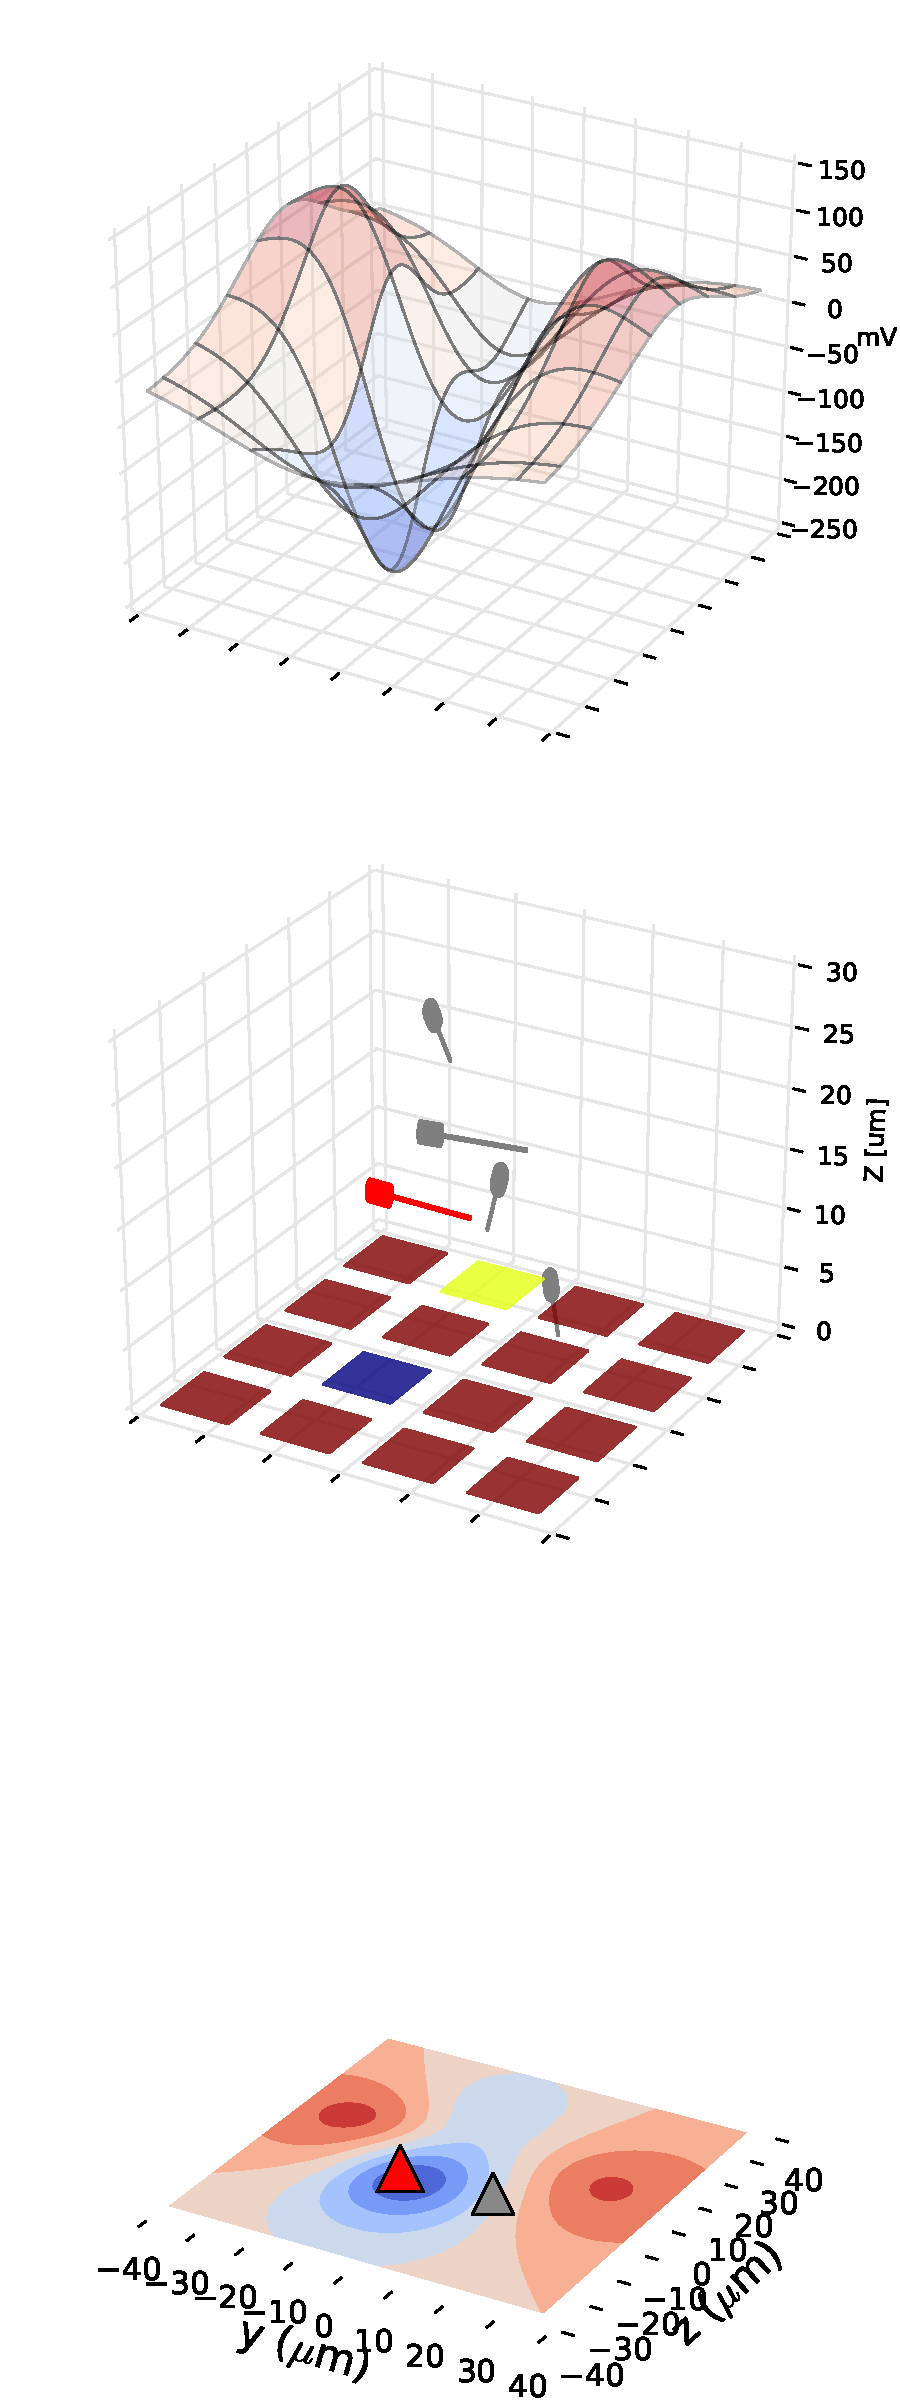
\includegraphics[scale=0.2]{Results_3d}
\par\end{centering}

\caption{\label{fig:neurons_and_field}\emph{Top:} Target neuron (red) and
surrounding neurons (gray) with MEA. Colors are current amplitudes.
\emph{Middle:} Potential surface at \emph{x }= 15 \textgreek{m}m.
\emph{Bottom: }2D projection of potential, MEA, and neurons.}
\end{figure}


First, let us analyze one of the random \emph{scenarios}. The top
panel of Fig. \ref{fig:neurons_and_field} shows the 3D position and
direction of the neurons, as well as the MEA electrode locations.
The larger cylinders represent the somas, while the narrower ones
are the axon hillock direction. It can be noticed how the configuration
can be intricated and tangled, depending on the relative alignment
between the target and surrounding neurons and their relative distance.
The colors on the MEA depicts the intentisies of the applied currents.
In the central panel the potential generated by the MEA on the plane
(15 \textgreek{m}m,\emph{ x}, \emph{y}) is displayed as a 3D surface.
It can be appreciated how troughs and hills are shaped so that the
target neuron falls in a positive AF region, while the surrounding
neurons do not. The bottom panel shows a contour plot of the field
and the projection of the neurons on the MEA plane (0, \emph{x}, \emph{y})
and the 2D projection o the neurons on the same plane. 
\begin{figure}[b]
\begin{centering}
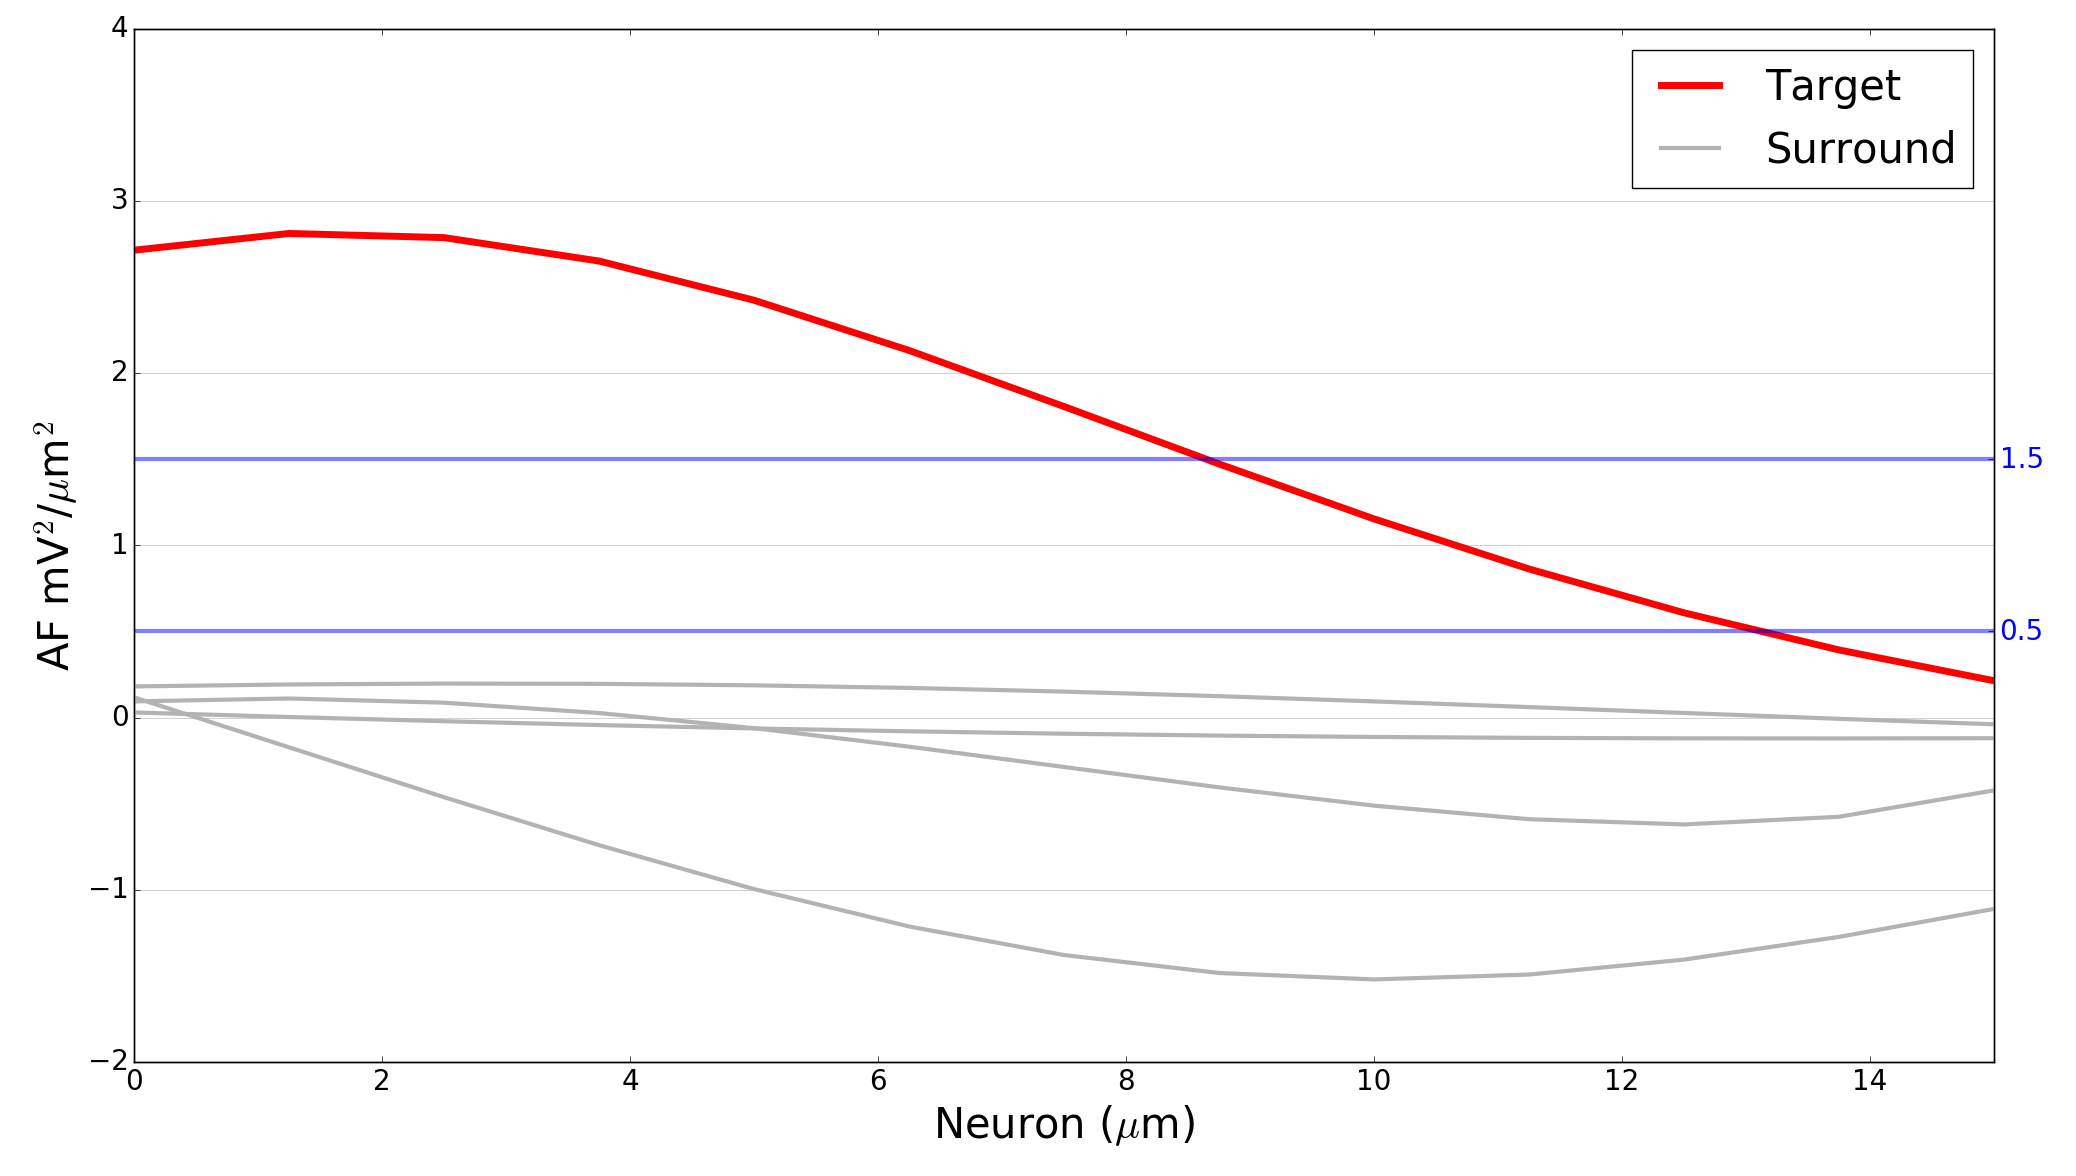
\includegraphics[scale=0.15]{figure_2_crop}
\par\end{centering}

\caption{ \label{fig:af_trg_surr}AF trend along the neuron for the target
neuron (red) and the surrounding neurons (gray). The blue horizontal
lines are the activation and non-activation threshold (1.5 mV$^{2}$/\textgreek{m}m$^{2}$
and 0.5 mV$^{2}$/\textgreek{m}m$^{2}$, respectively)}


\end{figure}


Fig. \ref{fig:af_trg_surr} shows the trends of the AF for the target
neuron (red) and surrounding neurons (gray). It is clear that the
optimized spatial pattern, for this \emph{scenario}, is able to pull
the AF above the activation threshold almost for all the points of
the target neuron and to keep the non-target neurons' AF below the
threshold with a relatively large margin. However, it should be noticed
that there is a lot of variability among \emph{scenarios} and not
always the GA achieves the objectives. Nevertheless, even if the threshold
is not reached, the target neuron's AF is pulled as high as possible
as long as the surrounding neurons are kept at rest.


\subsection{Genetic Algorithm, Monopolar, and Bipolar Comparison}

The performance of stimulation concerns both the activation of the
target neuron and the non-activation of the non-target neurons. In
each scenario, the AF is computed on 15 points (every 1 \textgreek{m}m),
hence for every \emph{scenario }different metrics are computed from
the AF of each neuron. In Table \ref{tab:trg} the average of each
of these values among the entire 1000 \emph{scenarios }for the target
neuron is shown. The mean, median, and maximum values are smaller
for GA than for MONO and BI, implying that the AF trend is overall
lower for GA. The last column shows the percentage of \emph{scenarios}
in which the maximum AF value is above the activation threshold.The
GA pattern is able to stimulate the target neuron in 100 \% of the
cases, more reliably than the monopolar (81.9 \%) and bipolar (77
\%) approaches.

\begin{table}[t]
\begin{centering}
\begin{tabular}{lcccccc}
\textbf{Target} & {\scriptsize{}mean} & {\scriptsize{}median} & {\scriptsize{}max} & {\scriptsize{}min} & {\scriptsize{}sd} & {\scriptsize{}\%max>threshold}\tabularnewline
\hline 
\noalign{\vskip\doublerulesep}
{\scriptsize{}GA} & 0.76 & 0.76 & 2.58 & -1.10 & {\footnotesize{}1.26} & \textbf{\footnotesize{}100\%}\tabularnewline
\noalign{\vskip\doublerulesep}
{\scriptsize{}MONO} & 1.68 & {\footnotesize{}1.20} & 5.49 & -1.05 & 2.30 & {\footnotesize{}81.9\%}\tabularnewline
\noalign{\vskip\doublerulesep}
{\scriptsize{}BI} & 1.28 & 0.98 & 5.65 & -2.52 & 2.80 & {\footnotesize{}77\%}\tabularnewline
\end{tabular}\medskip{}

\par\end{centering}

\caption{\label{tab:trg} Performance on target neuron. Mean, median, max,
min, and sd are the average over the 1000 \emph{scenarios }of the
AF along the target neuron }
\end{table}


In order to evaluate the selectivity of the stimulation we considered
the surrounding neuron with the highest AF. If a non-target neuron's
AF gets close to the activation threshold, then it is likely that
a spurious spike is generated. In Table \ref{tab:surr} the statistics
of the maximum values among the non-target neurons are displayed.
The values are overall smaller for the GA approach, especially the
maximum value of the AF. From the last column, which shows the percentage
of surrounding neurons (in this case all the surrounding neurons are
considered, not only the one with highest AF) whose AF reaches the
activation threshold of 1.5 mV$^{2}$/\textgreek{m}m$^{2}$, it can
be appreciated how the GA is more robust than MONO and BI, since it
pulls non-target neurons above threshold only in 0.5 \% of the cases,
compared to the 19.8 \% of the monopolar approach and the 26.9 \%
of the bipolar one.

\begin{table}[b]
\begin{centering}
\begin{tabular}{lcccccc}
\textbf{Non-Targe}t & {\scriptsize{}mean} & {\scriptsize{}median} & {\scriptsize{}max} & {\scriptsize{}min} & {\scriptsize{}sd} & {\scriptsize{}\%max>threshold}\tabularnewline
\hline 
\noalign{\vskip\doublerulesep}
{\scriptsize{}GA} & {\footnotesize{}0.13} & {\footnotesize{}0.14} & {\footnotesize{}0.27} & {\footnotesize{}0.05} & {\footnotesize{}0.30} & \textbf{\footnotesize{}0.5\%}\tabularnewline
\noalign{\vskip\doublerulesep}
{\scriptsize{}MONO} & {\footnotesize{}0.51} & {\footnotesize{}0.47} & {\footnotesize{}1.38} & {\footnotesize{}0.11} & {\footnotesize{}0.58} & {\footnotesize{}19.8\%}\tabularnewline
\noalign{\vskip\doublerulesep}
{\scriptsize{}BI} & {\footnotesize{}0.53} & {\footnotesize{}0.54} & {\footnotesize{}1.63} & {\footnotesize{}0.08} & 1.11 & {\footnotesize{}26.9\%}\tabularnewline
\end{tabular}\medskip{}

\par\end{centering}

\caption{\label{tab:surr} Performance on non-target neurons. The values refer
to the surrounding neurons with the highest value for the different
metrics.}
\end{table}


Fig. \ref{fig:ga_mono_bi} displays the boxplots of the distributions
of the maximum surround AF (the same values shown in \ref{tab:surr}),
divided between the 3 approaches (GA, MONO, BI). The higher selectivity
and robustness of the GA stimulation is reflected in the less number
of outliers, which means that in less cases spurious spikes are generated.
Moreover, the values of the AF above the activation threshold (1.5
mV$^{2}$/\textgreek{m}m$^{2}$, blue horizontal line) are higher
for MONO and BI approach, due to their lower adaptation to the environment,
especially to the surrounding neurons' position.
\begin{figure}[t]
\begin{centering}
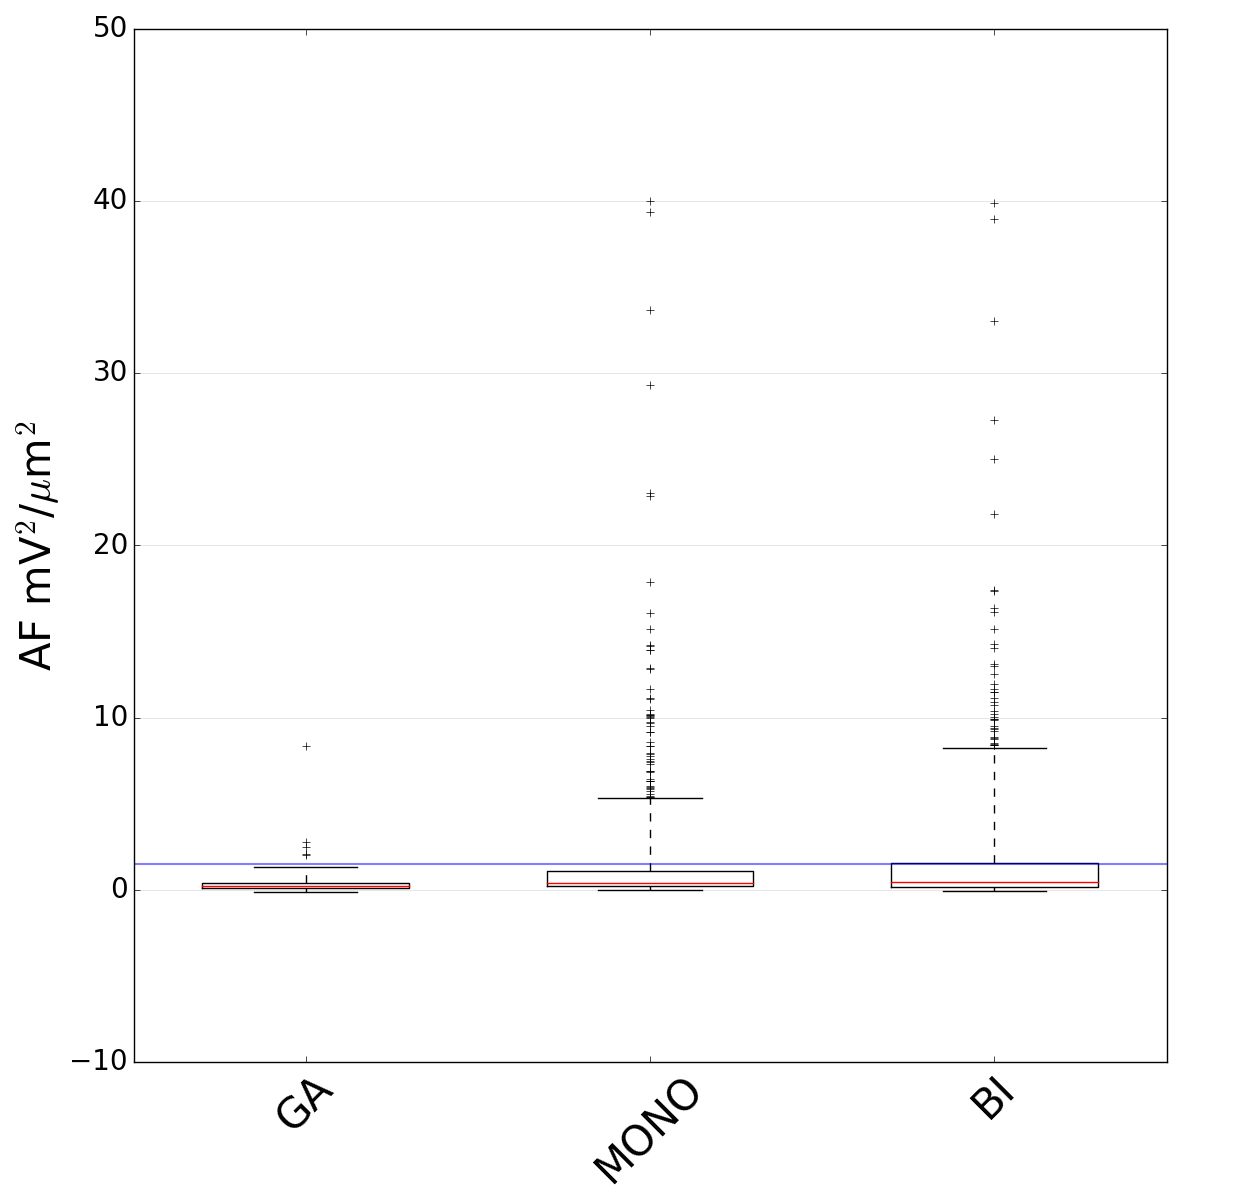
\includegraphics[scale=0.15]{figure_3_crop}
\par\end{centering}

\caption{\label{fig:ga_mono_bi}Boxplots of maximum AF on surrounding neurons
divided by stimulation approach (GA, MONO, BI). The blue horizontal
line is the activation threshold of 1.5 mV$^{2}$/\textgreek{m}m$^{2}$}


\end{figure}


It is interesting to analyze to output of the GA also in terms of
sparsity and energy efficiency. In 68.2 \% of the cases the GA outputs
a monopolar pattern, but it should be emphazised that the intensity
of the current is adapted to the scenario. In 92.5 \% of the cases,
instead, only 3 or less electrodes are involved in the spatial pattern.
The \emph{convergence} of the GA to a monopolar- or bipolar-like solution
when the \emph{scenario} is not too complex is ensured by the sparsity
and energy efficiency terms in the fitness function (Eq. \ref{eq:fitness}),
which tries to maximize the number of non-active electrode and to
minimize the current delivered from each electrode. On average, among
all 1000 \emph{scenarios}, the total amount of delivered current is
15.81 \textgreek{m}A, in between the monopolar (10 \textgreek{m}A)
and the bipolar (20 \textgreek{m}A) stimulation.


\section{Discussions and Conclusion\label{sec:Discussions-and-Conclusion}}

In this study we presented a novel approach to exploit the high density
of MEA for improving stimulation selectivity and adaptation. We showed
that the proposed method is more selective and robust than standard
monopolar and bipolar approaches, even if it would require more energy
consumption and a more complex control. 

In order to speed up the optimization and possibly make it implementable
also in an online setup, we used monopolar current source approximation
a simple model for the MEA. Clearly, the geometry of the electrodes
play an important role; hence, the error between the monopolar current
source approximation and a more accurate method, such as a Finite
Element Methods (which has been applied to MEA in \cite{joucla2013current}),
should be characterized for an \emph{a-posteriori }evaluation. 

Moreover, we assumed to be able to estimate the exact position of
the neurons' somas and to be able their axon hillock direction from
recorded data. This is definitely a strong assumption, but previous
studies showed that HD MEA are capable of providing such information
\cite{ruz2014localising}\cite{muller2015high}. Nevertheless, the
estimation error involved in this step should be evaluated as well,
and our future work will deal with the entire loop: from recorded
data, to position and direction estimation, to stimulation and evaluation
of the outcome on more complex neural models, as well as \emph{in-vivo}.

In conlusion, we introduced an optimization approach for neural stimulation
with HD MEA, which could lead to the capability of robustly targeting
single neurons with extra-cellular electrical stimulation.


\section{Acknowledgments}

Alessio Paolo Buccino, Tristan St�ber, and Solveig N�ss are doctoral
fellows in the Simula-UCSD-University of Oslo Research and PhD training
(SUURPh) program, an international collaboration in computational
biology and medicine funded by the Norwegian Ministry of Education
and Research.

\bibliographystyle{IEEEtran}
\bibliography{references2}

\end{document}
